\documentclass{beamer}
 
\usepackage[utf8]{inputenc}
 
 
%Information to be included in the title page:
\title{Part Two: \\Decoding: The Viterbi Algorithm}
\author{Zihao Zhu, Gangze Li, Yufeng Xie}
\institute{Tsinghua University}
\date{\today}
\setbeamertemplate{footline}[frame number]
\usepackage{color}
\usepackage{graphicx}
\usepackage{wallpaper}
\usepackage{hyperref}
\usepackage{subfigure}
\usepackage{stackengine}
\usepackage{scalerel}
\usepackage{xcolor}
\newcommand\dangersign[1][2ex]{%
  \renewcommand\stacktype{L}%
  \scaleto{\stackon[1.3pt]{\color{red}$\triangle$}{\tiny !}}{#1}%
}
\begin{document}
 
\frame{\titlepage}
 


\begin{frame}
\frametitle{Decoding}
\quad
\fbox{%
  \parbox{\textwidth}{%
    
    Decoding: Given as input an HMM $\lambda=(A, B)$ and a sequence of observations $O=o_{1}, o_{2}, \ldots, o_{T}$, find the most probable sequence of states $Q=q_{1} q_{2} q_{3} \ldots q_{T}$.
  }%
}

% \begin{figure}[H]
%     \centering
%     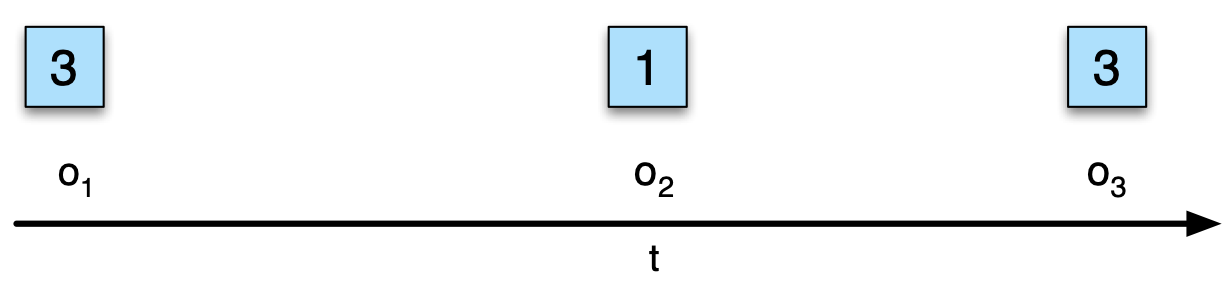
\includegraphics[width=0.7\textwidth]{img/1.png}
%     \end{figure}

\begin{figure}[htbp]
    \centering
    \subfigure[observations]{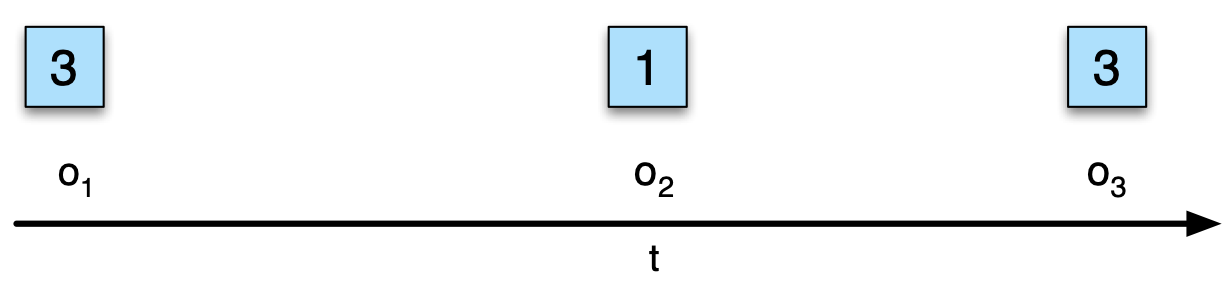
\includegraphics[width=4cm]{img/1.png}}
    \subfigure[$\lambda=(A, B)$]{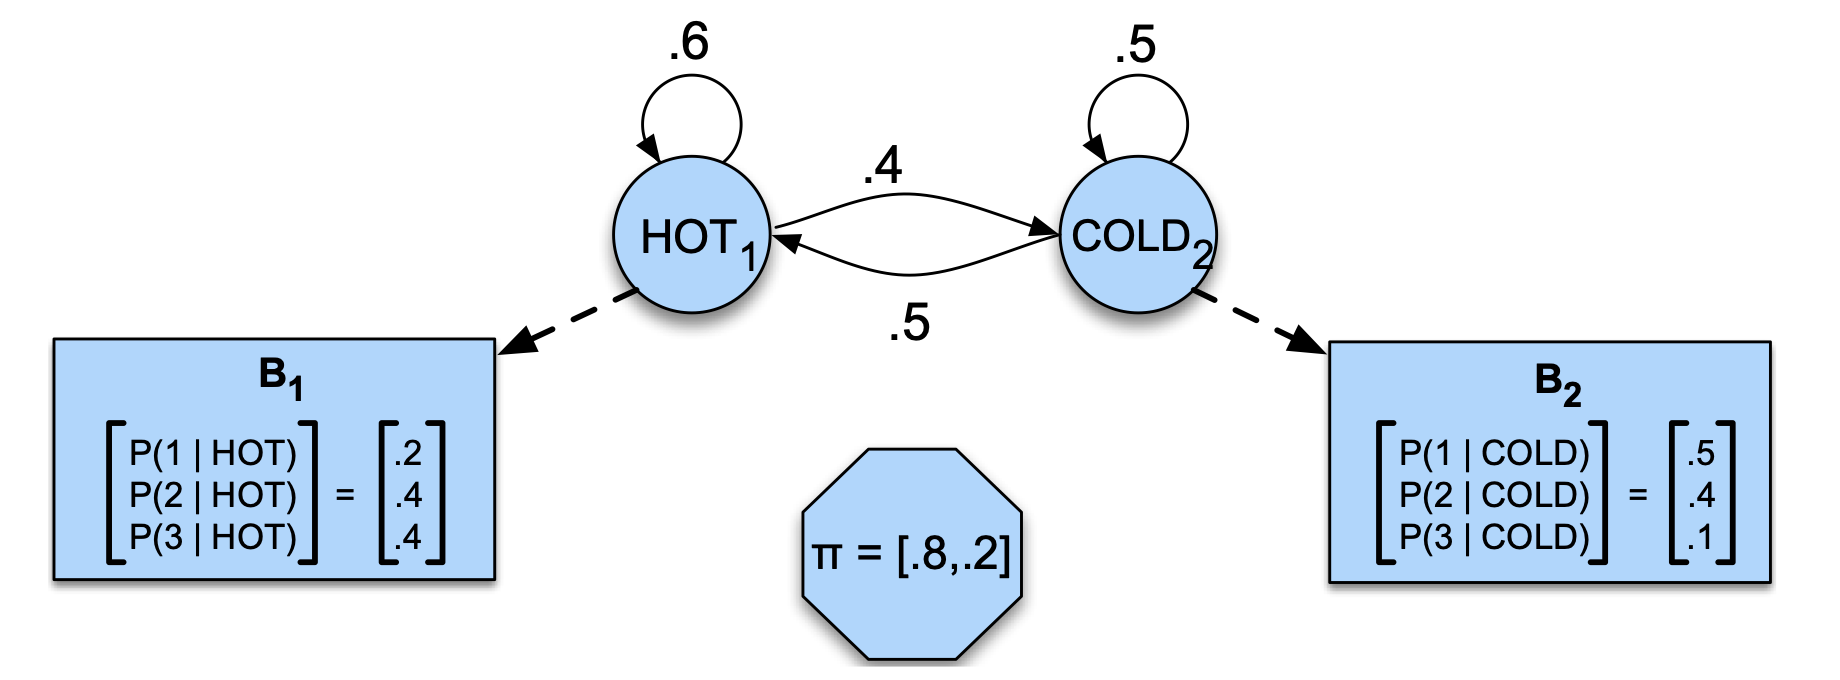
\includegraphics[width=4cm]{img/14.png}}
    \quad
    \subfigure[hidden weather sequence]{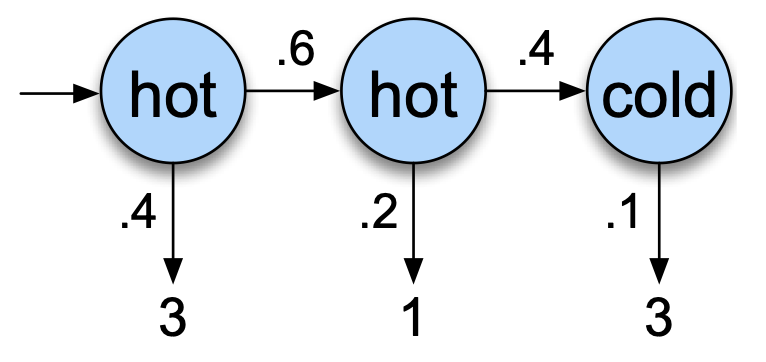
\includegraphics[width=3cm]{img/15.png}}
    \caption{In the ice-cream domain, given a sequence of ice-cream observations 3 1 3 and an HMM, the task of the decoder is to find the best hidden weather sequence (H H H).}
    % \begin{minipage}[t]{0.48\textwidth}
    % \centering
    % 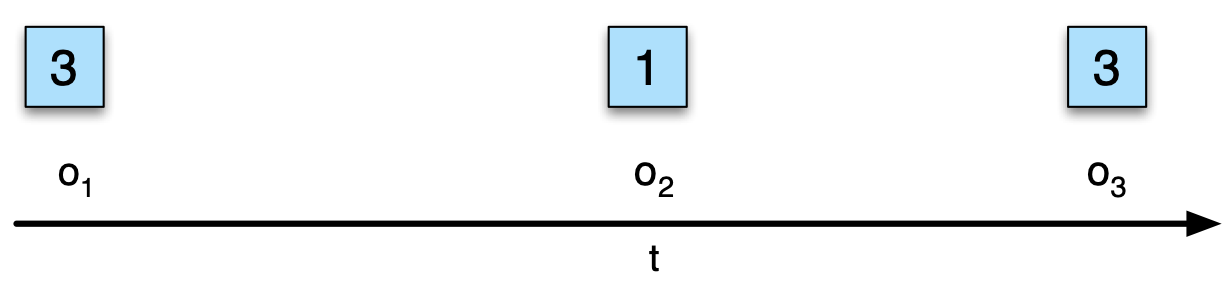
\includegraphics[width=4cm]{img/1.png}
    % \caption{observations}
    % \end{minipage}
    % \begin{minipage}[t]{0.48\textwidth}
    % \centering
    % 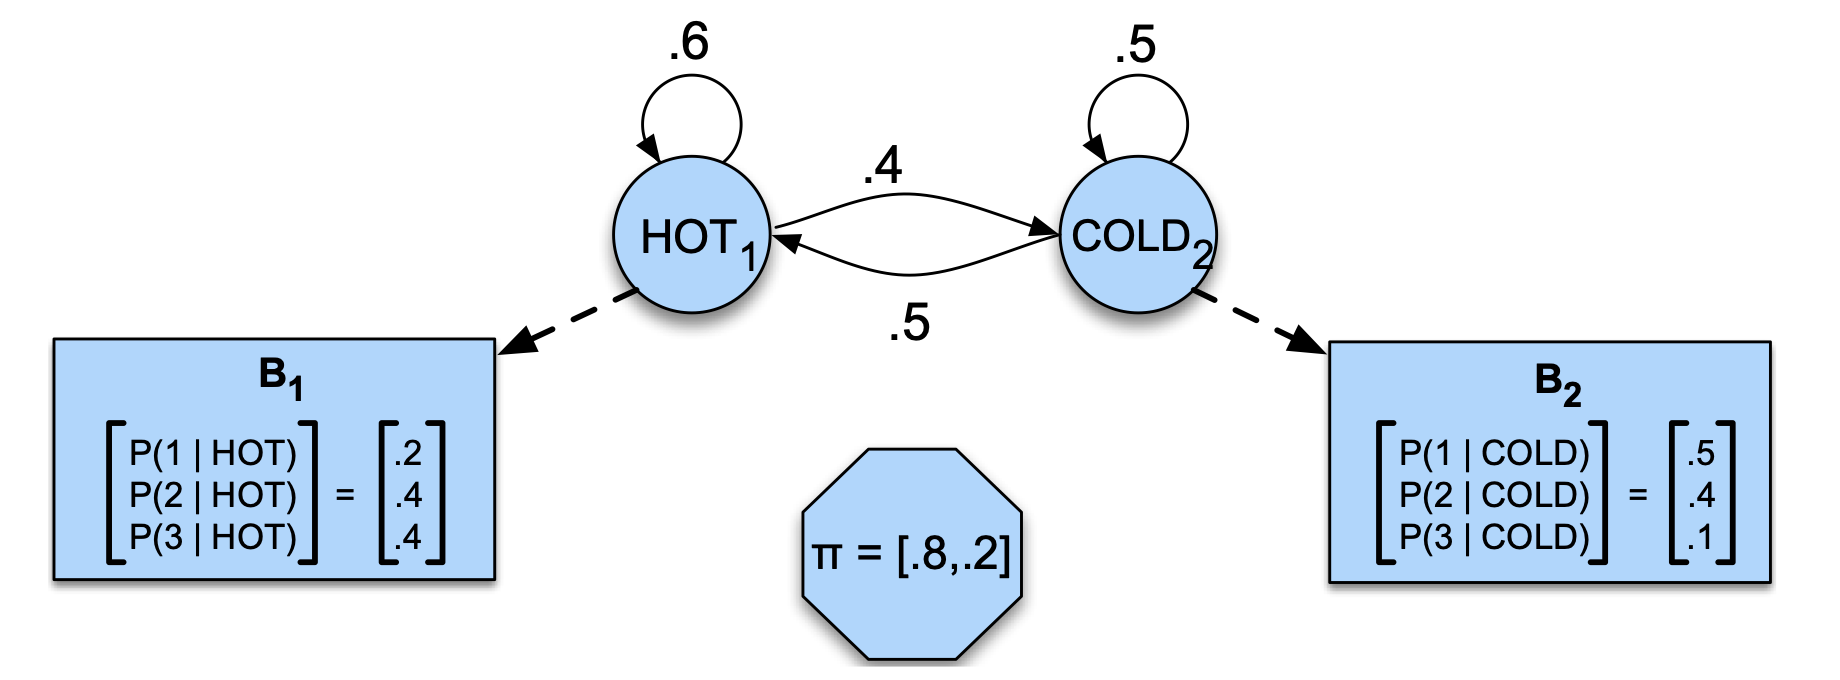
\includegraphics[width=6cm]{img/14.png}
    % \caption{$\lambda=(A, B)$}
    % \end{minipage}
    \end{figure}

\end{frame}

\begin{frame}
    %\addtocounter{framenumber}{-2}%
    \frametitle{Problem}
    \begin{itemize}
        \item One possibility 
        \begin{itemize}
            \item For each hidden state sequence $Q$
            \begin{itemize}
                \item HHH, HHC, HCH, etc.
            \end{itemize}
            \item Compute $P(O|Q)$
            \item Pick the highest one
        \end{itemize}
        \item \dangersign[5ex]  likelihood: $N^T$ \\a set of $N$ states, a sequence of $T$ observations
        \item Instead
        \begin{itemize}
            \item \color{red}Viterbi algorithm
        \end{itemize}
    \end{itemize}
    

    \end{frame}
\begin{frame}
    \frametitle{Problem}
    \begin{figure}[H]
        \centering
        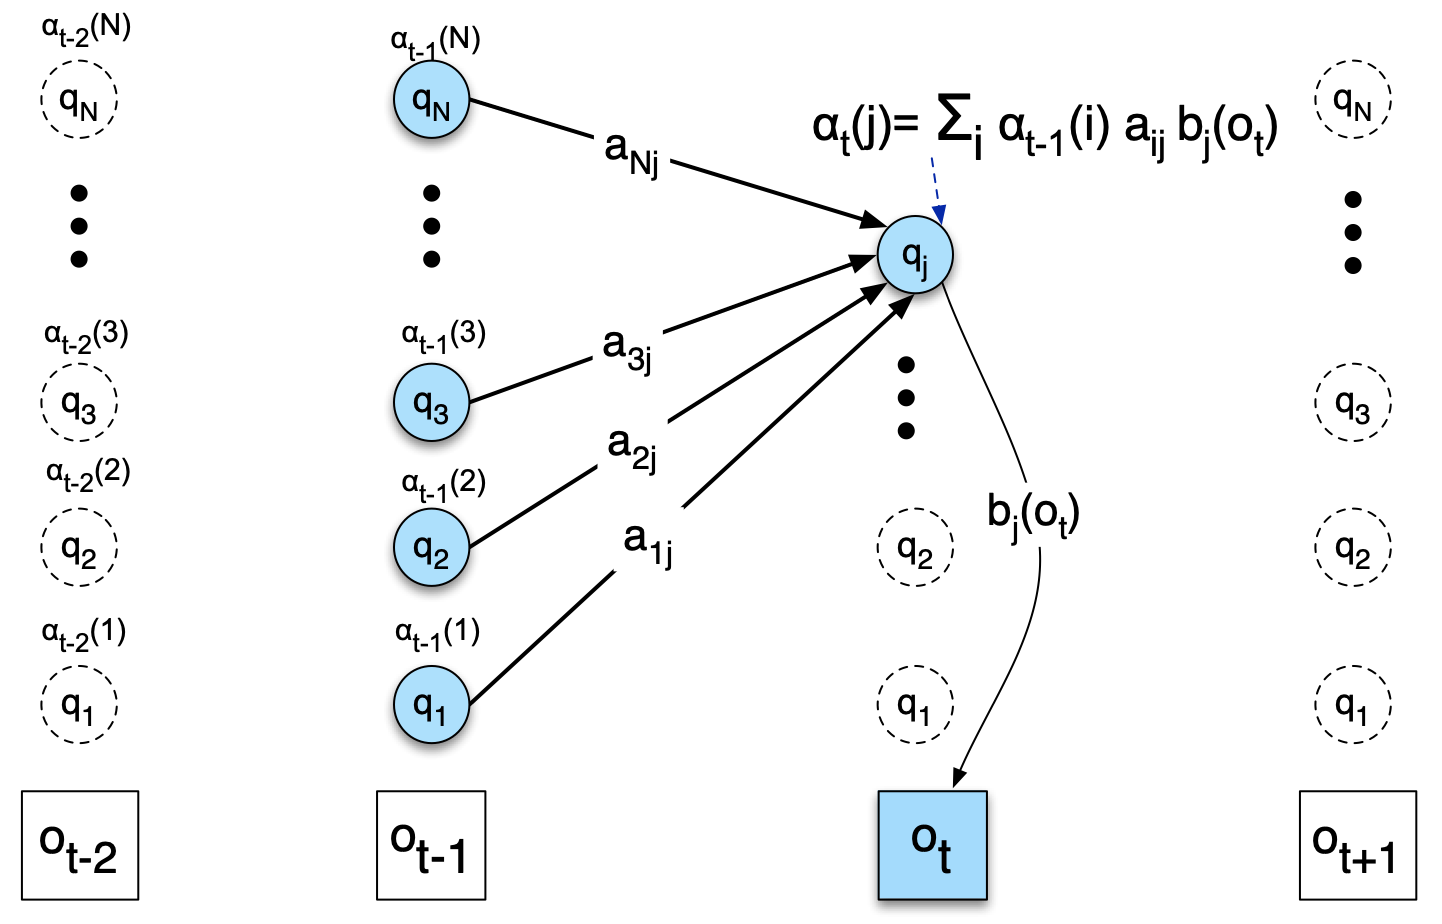
\includegraphics[width=0.8\textwidth]{img/16.png}
        \caption{exponentially large number of state sequences! \footnote{example from \cite{Jurafsky:2009:SLP:1214993}}}

        \end{figure}
\end{frame}

\begin{frame}
    \frametitle{Viterbi algorithm}
    \begin{itemize}
        \item The Viterbi algorithm is a dynamic programming algorithm for finding the most likely sequence of hidden states.
        \item We want to compute the joint probability of the observation sequence together with the best state sequence.
        \begin{itemize}
            \item     $
            v_{t}(j)=P\left(q_{0}, q_{1}, \ldots, q_{t-1}, o_{1}, o_{2}, \ldots, o_{t}, q_{t}=j | \lambda\right)
            $
            \item $
            \alpha_{t}(j)=P\left(o_{1}, o_{2} \ldots o_{t}, q_{t}=j | \lambda\right)
            $
        \end{itemize}
    \end{itemize}

\end{frame}

\begin{frame}
    \frametitle{The forward trellis}
    compute the total observation likelihood for the ice-cream events 3 1 3
    \begin{figure}[H]
    \centering
    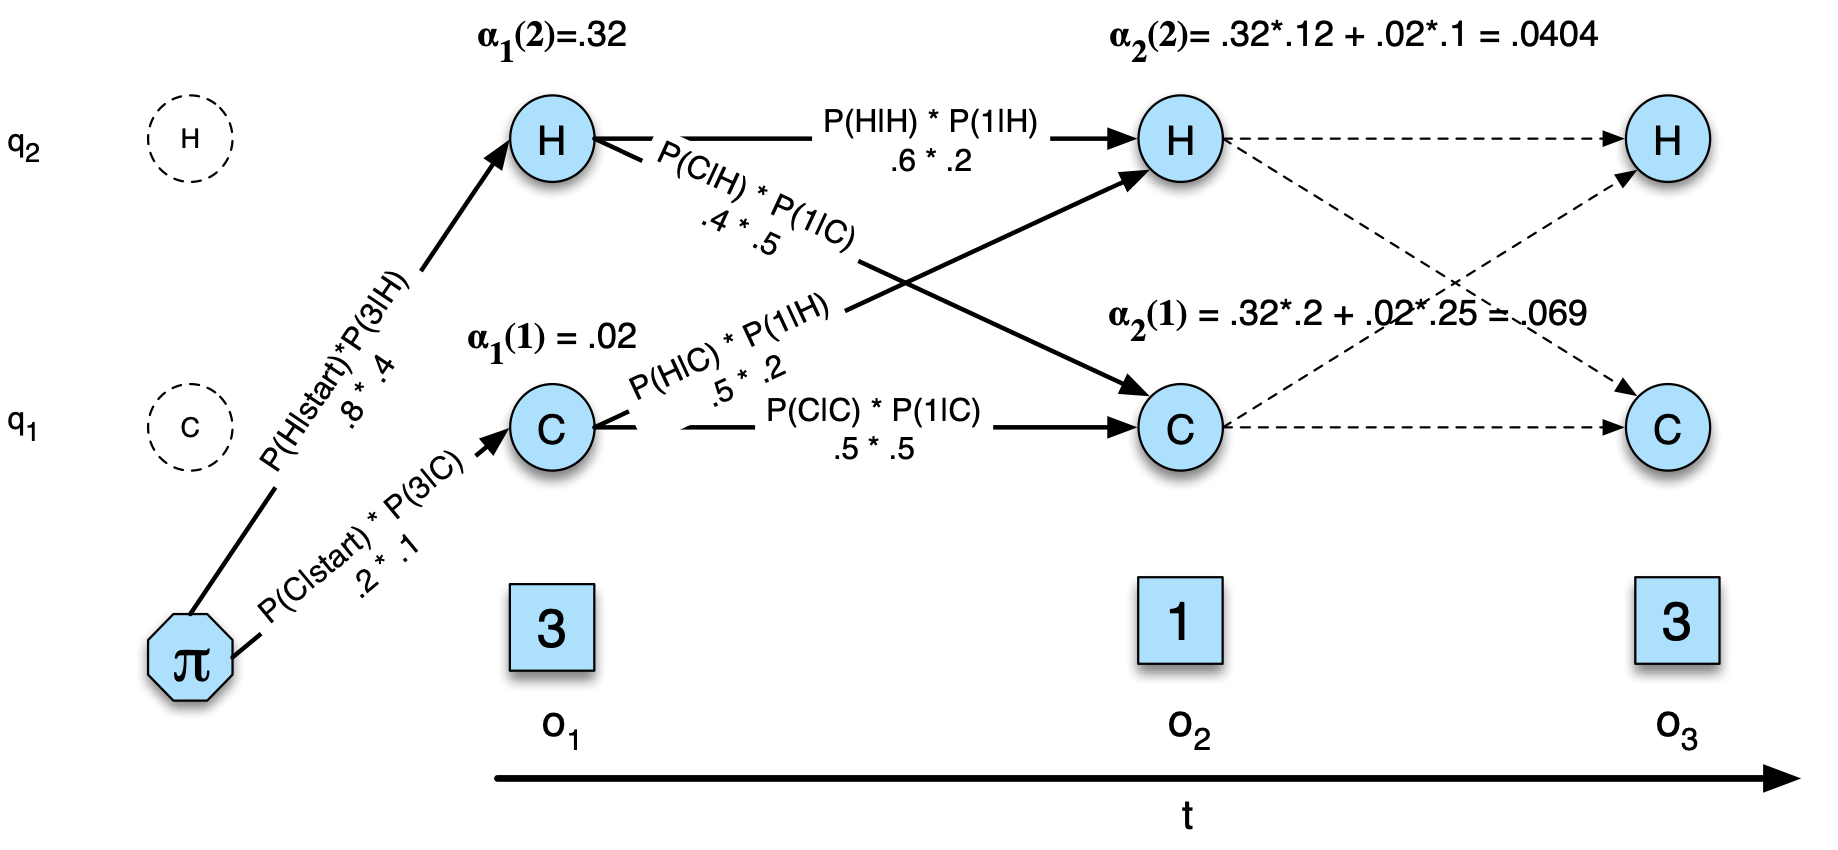
\includegraphics[width=\textwidth]{img/17.png}
    \end{figure}
    $
            \alpha_{t}(j)=P\left(o_{1}, o_{2} \ldots o_{t}, q_{t}=j | \lambda\right)
            $
    \end{frame}

\begin{frame}
\frametitle{Viterbi algorithm}
the computation of $v_t(j)$ for two states at two time steps
\begin{figure}[H]
\centering
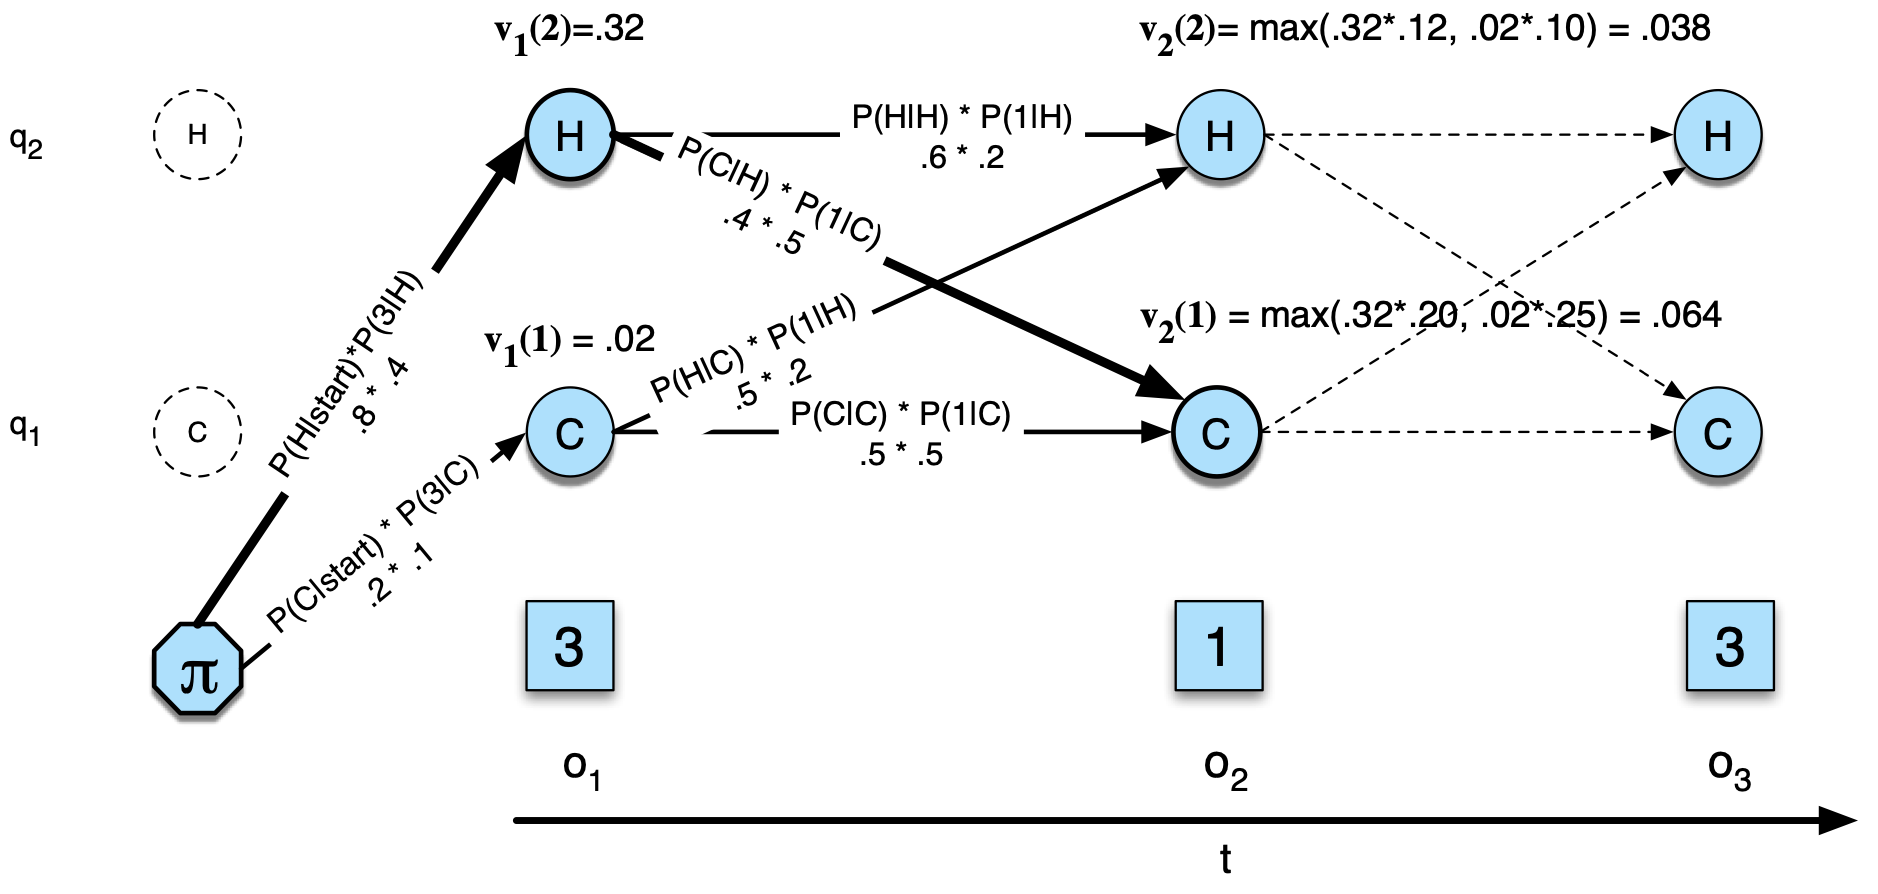
\includegraphics[width=\textwidth]{img/2.png}
\end{figure}
$
            v_{t}(j)=P\left(q_{0}, q_{1}, \ldots, q_{t-1}, o_{1}, o_{2}, \ldots, o_{t}, q_{t}=j | \lambda\right)
            $
\end{frame}

\begin{frame}
    \frametitle{Viterbi algorithm}
    \begin{itemize}
        \item The computation in each cell follows $
        v_{t}(j)=\max _{1 \leq i \leq N-1} v_{t-1}(i) a_{i j} b_{j}\left(o_{t}\right)
        $
        \item The resulting probability expressed in each cell is $
        v_{t}(j)=P\left(q_{0}, q_{1}, \ldots, q_{t-1}, o_{1}, o_{2}, \ldots, o_{t}, q_{t}=j | \lambda\right)
        $
    \end{itemize}
    
\end{frame}
% \begin{frame}
%     \frametitle{Left to right, filling out the trellis}
    
% \end{frame}

\begin{frame}
    \frametitle{the Viterbi backtrace}
    \begin{figure}[H]
        \centering
        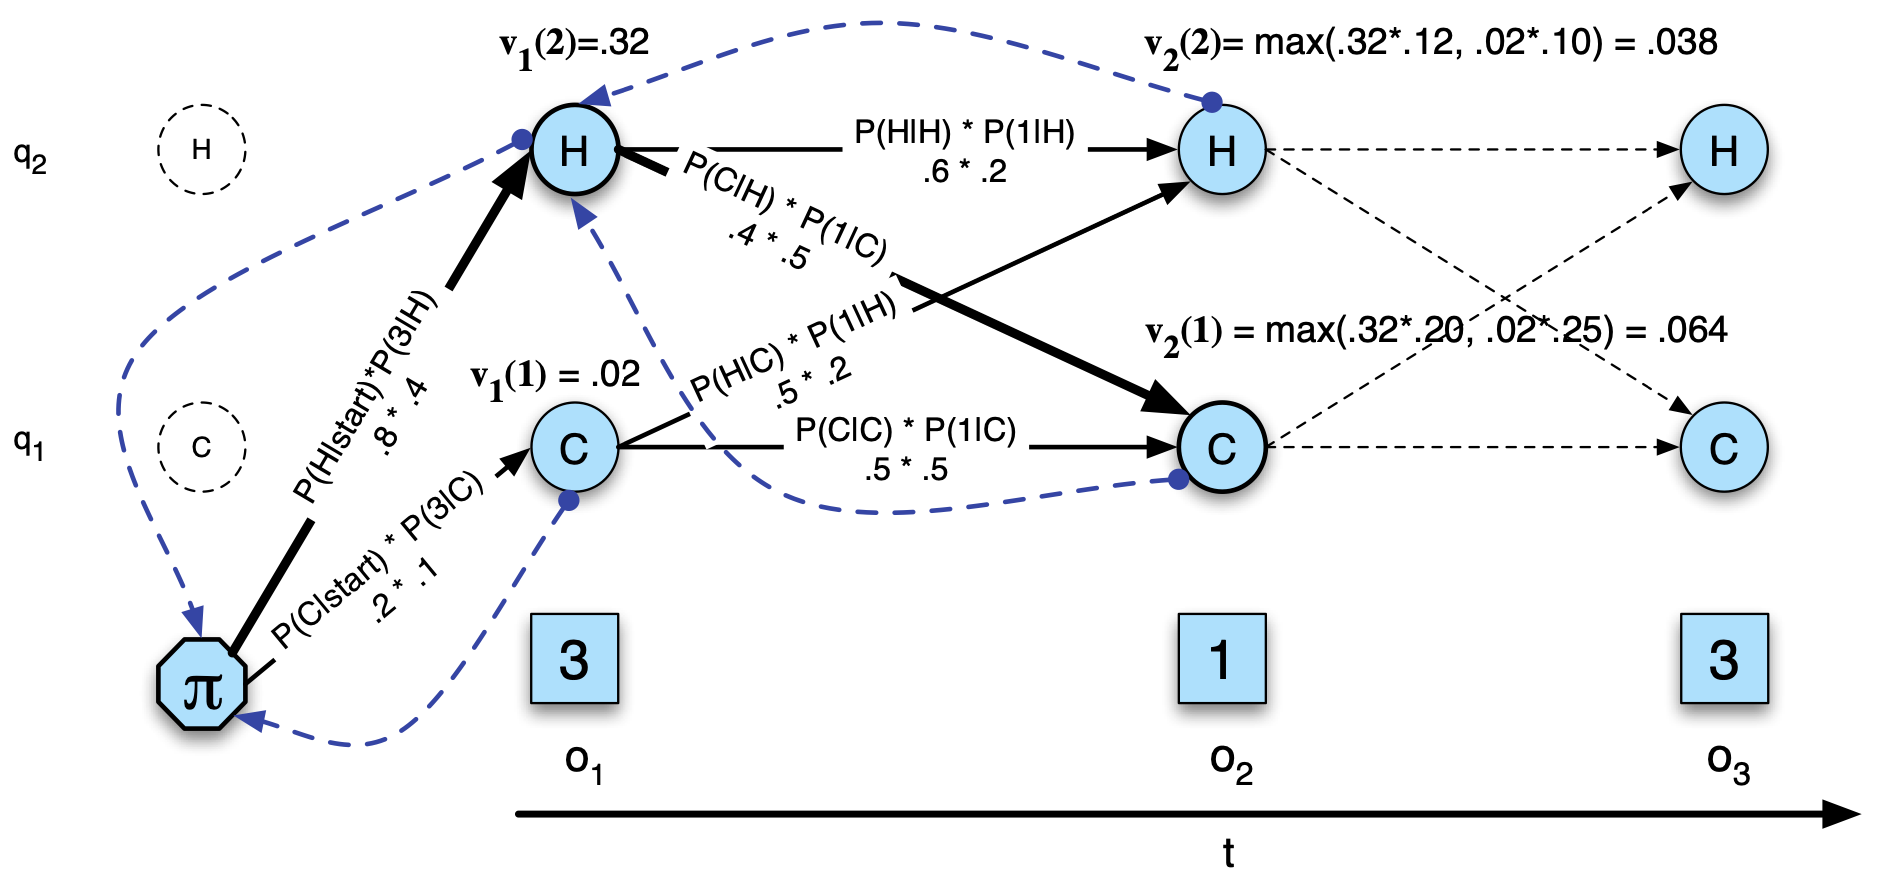
\includegraphics[width=\textwidth]{img/4.png}
        \caption{The Viterbi trellis for computing the best path through the hidden state space for the ice-cream eating events 3 1 3.}
        \end{figure}
\end{frame}
\begin{frame}
    \frametitle{Viterbi recursion}
\begin{itemize}
    \item Initialization $$
\begin{aligned} v_{1}(j) &=\pi_{j} b_{j}\left(o_{1}\right) & & 1 \leq j \leq N \\ b t_{1}(j) &=0 & & 1 \leq j \leq N \end{aligned}
$$
\item Recursion $$
\begin{aligned} v_{t}(j) &=\max_{i=1}^{N} v_{t-1}(i) a_{i j} b_{j}\left(o_{t}\right) ; \quad 1 \leq j \leq N, 1<t \leq T \\ b t_{t}(j) &={\operatorname{argmax}} ^{N}_{i=1} v_{t-1}(i) a_{i j} b_{j}\left(o_{t}\right) ; \quad 1 \leq j \leq N, 1<t \leq T \end{aligned}
$$
\item Termination $$
\begin{array}{c}{\text { The best score: } P * =\max _{i=1}^{N} v_{T}(i)} \\ {\text { The start of backtrace: } q_{T^{*}}={\operatorname{argmax}} ^{N}_{i=1} v_{T}(i)}\end{array}
$$
\end{itemize}
\end{frame}
\begin{frame}
    \frametitle{Pseudocode}
    \begin{figure}[H]
        \centering
        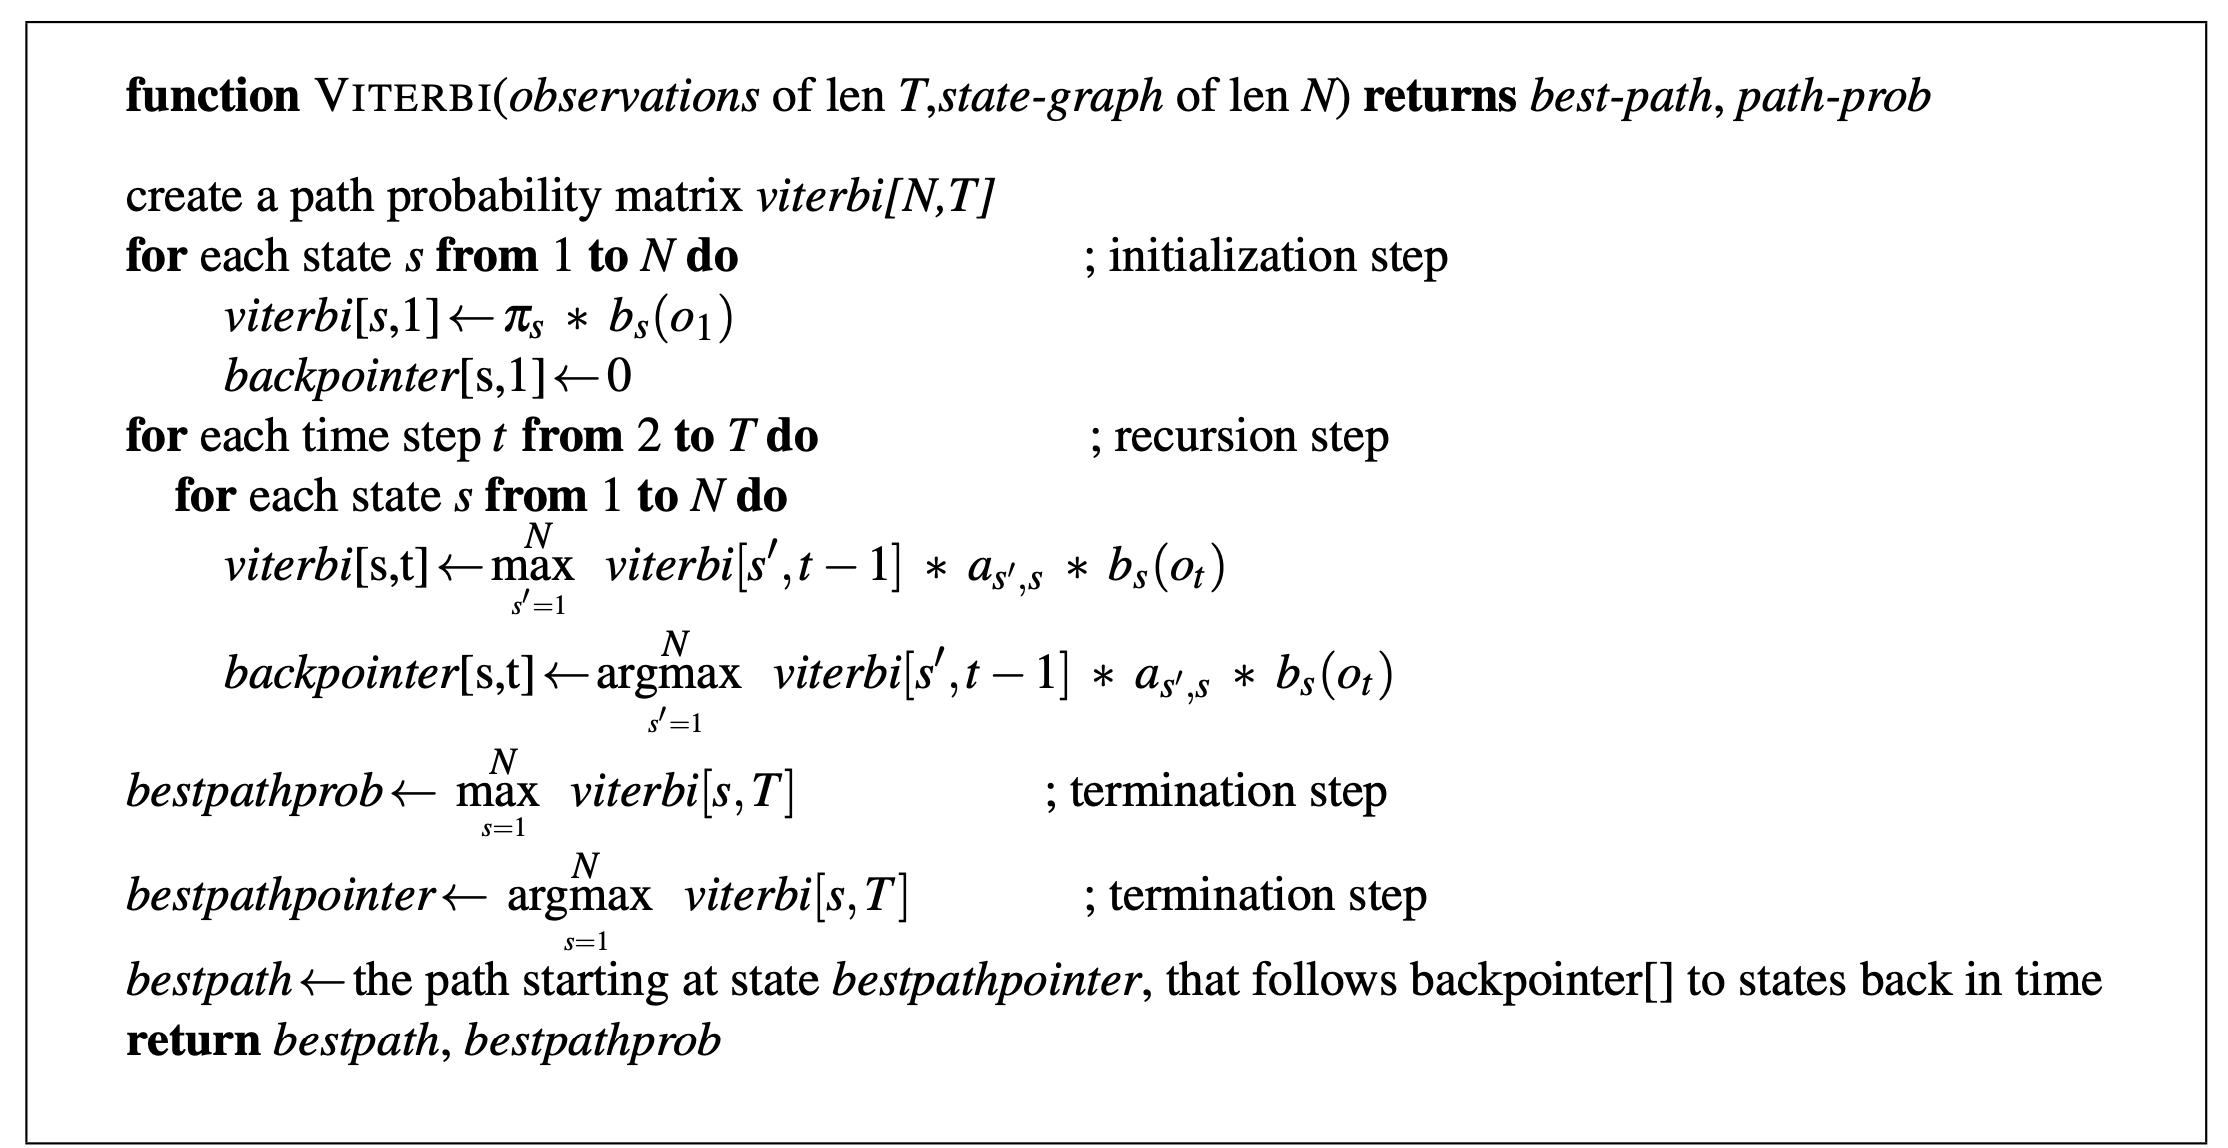
\includegraphics[width=\textwidth]{img/3.png}
        \end{figure}
\end{frame}
\begin{frame}
    \frametitle{Three fundamental problems \cite{rabiner1989tutorial}}
    \begin{itemize}
        \item {\color{gray}\textbf{Problem 1 (Likelihood)} Given an HMM $λ = (A, B)$ and an observation sequence $O$, determine the likelihood $P(O |\lambda)$.}
        \item \textbf{Problem 2 (Decoding)} Given an observation sequence $O$ and an HMM $λ = (A, B)$, discover the best hidden state sequence $Q$.
        \item {\color{gray}\textbf{Problem 3 (Learning)} Given an observation sequence $O$ and the set of states in the HMM, learn the HMM parameters $A$ and $B$.}
    \end{itemize}

\end{frame}
\begin{frame}
    \ThisCenterWallPaper{0.73}{img/5.png}
    \frametitle{Application\footnote{from the \href{http://hollywood.mit.edu/GENSCANinfo.html}{link}}}
    
    \begin{figure}[T]
        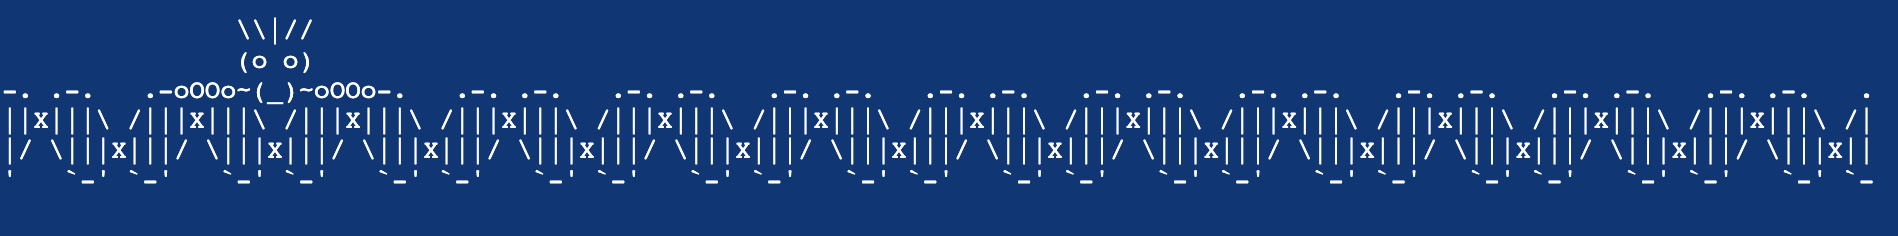
\includegraphics[width=0.8\textwidth]{img/5.png}
        \end{figure}
    \begin{figure}[T]
        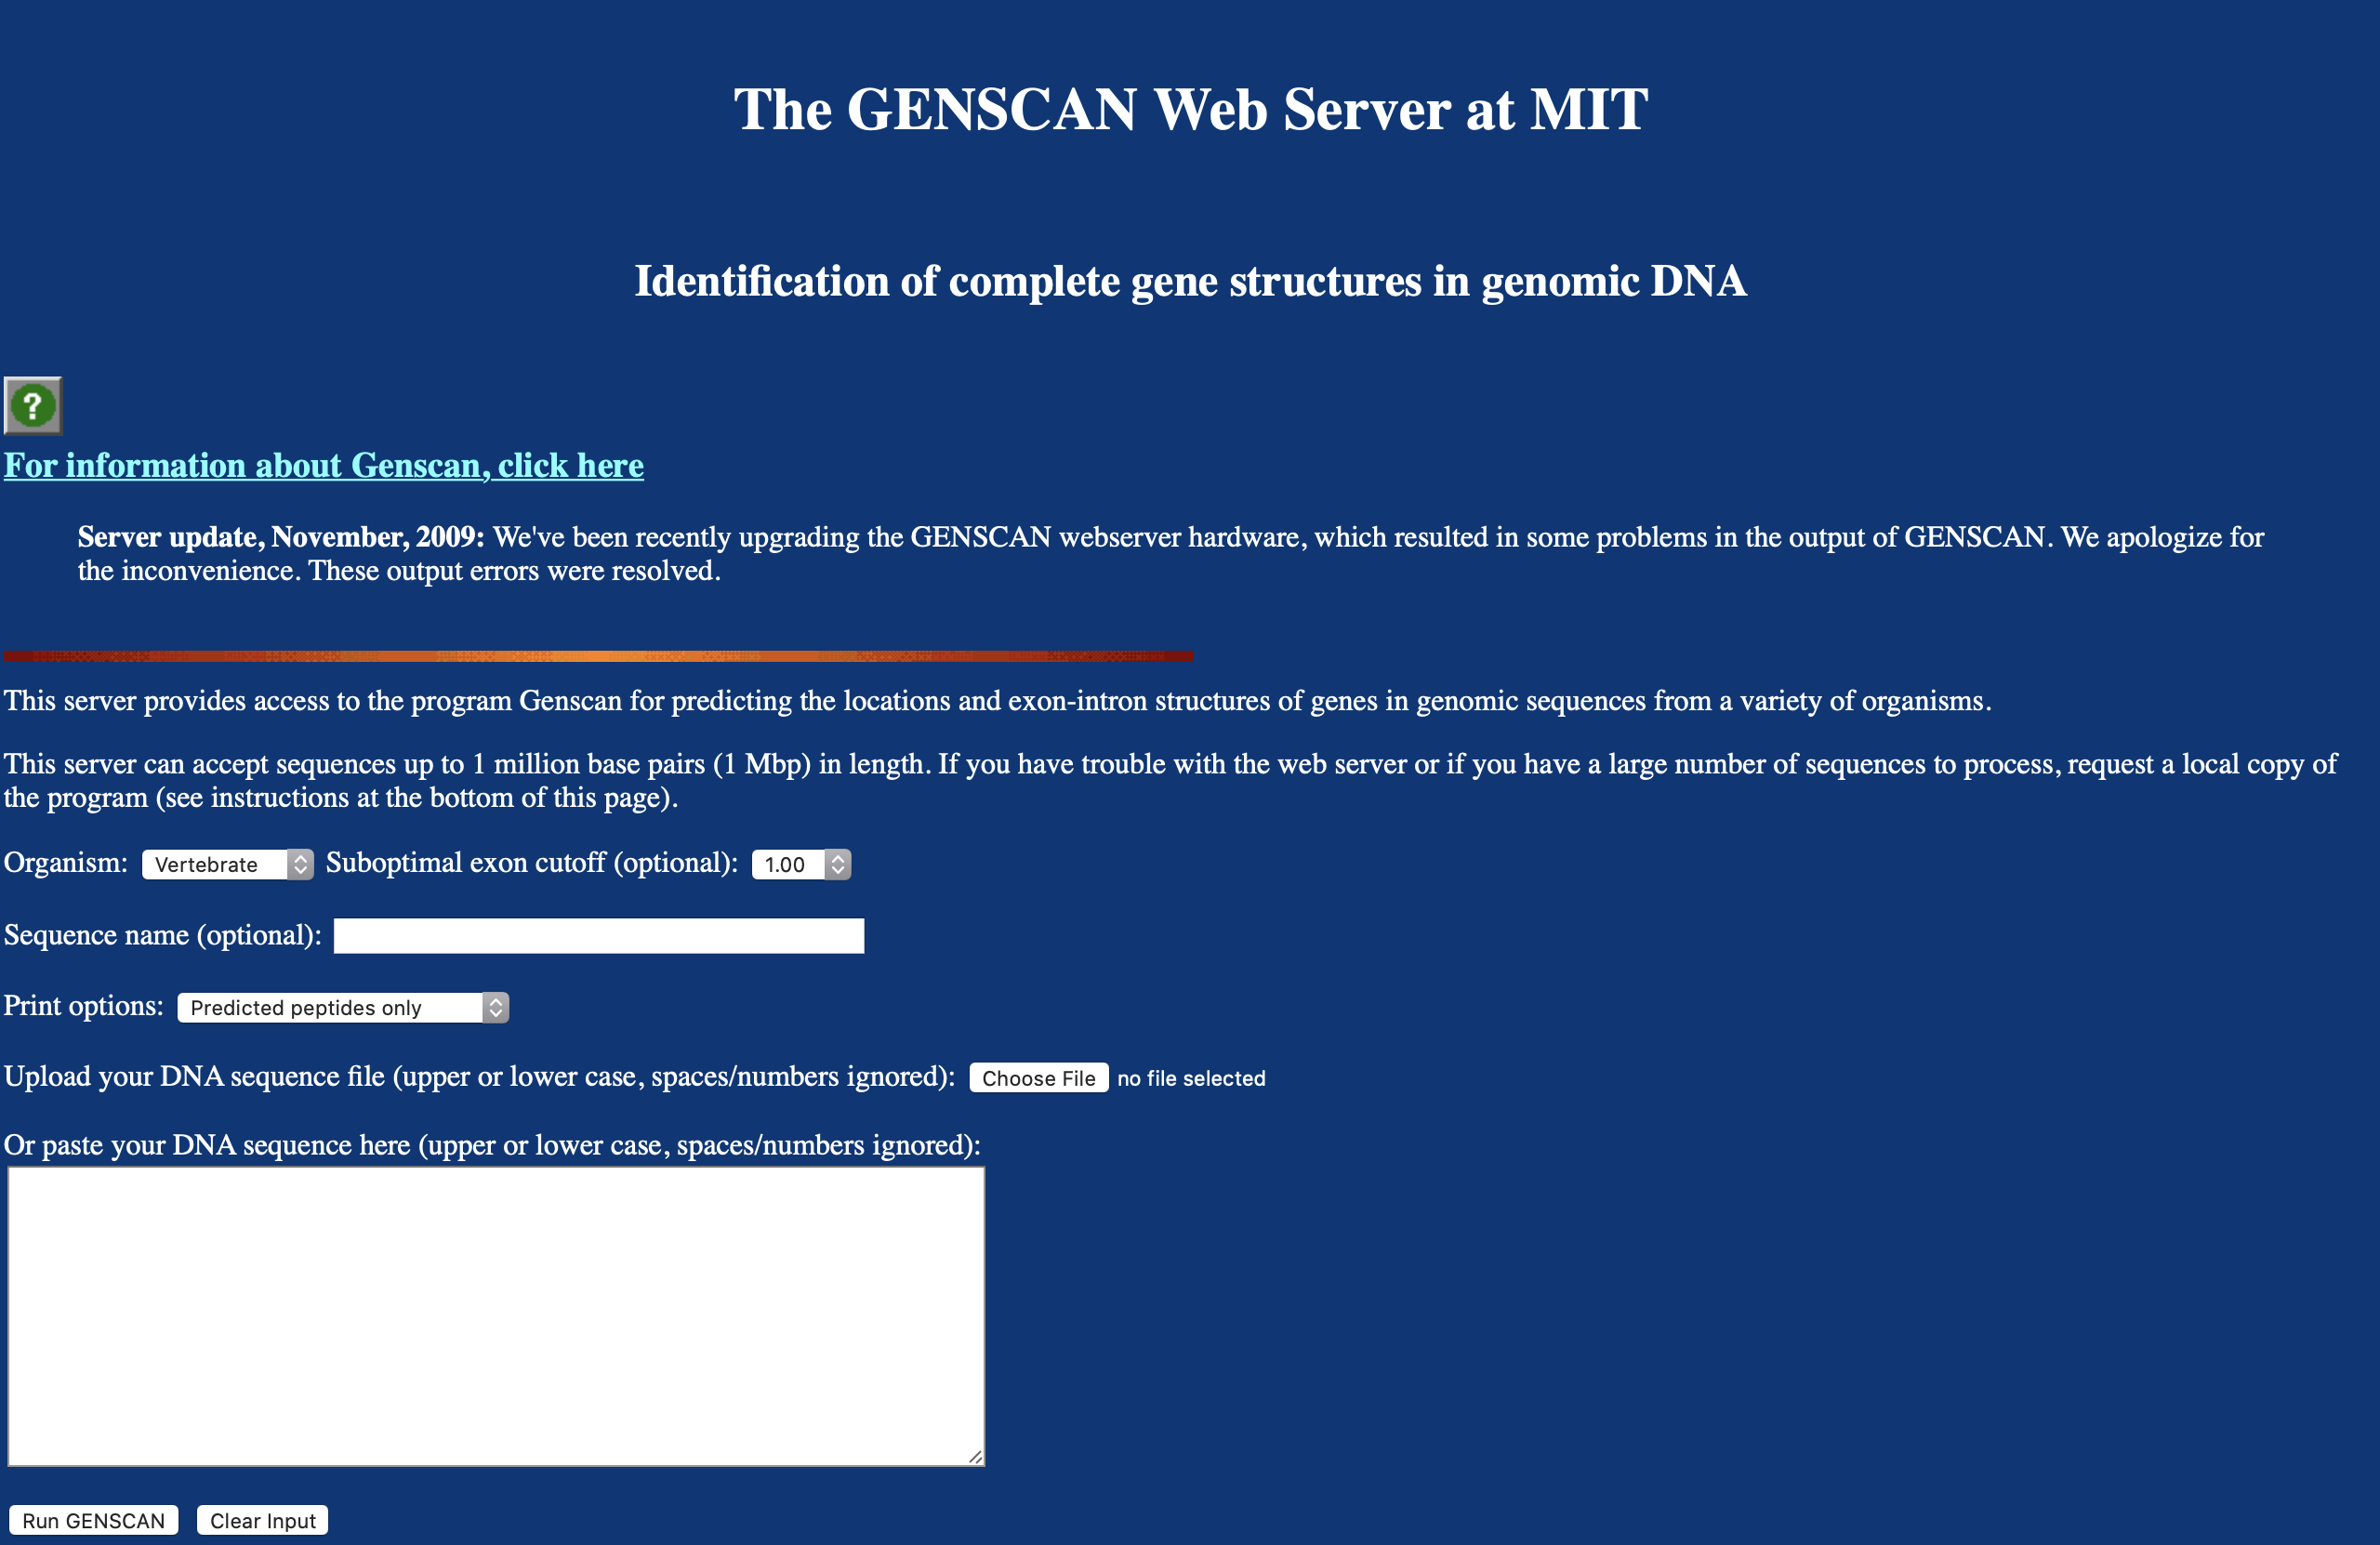
\includegraphics[width=0.8\textwidth]{img/6.png}
        \end{figure}

    \end{frame}
\begin{frame}
    \frametitle{GENSCAN}
    GENSCAN was developed by Chris Burge in the research group of Samuel Karlin, Department of Mathematics, Stanford University \cite{burge1997prediction,salzberg1998modeling}. 

    Burge and Karlin in their gene finding computer program GENSCAN used a three-periodic (inhomogeneous) fifth order Markov chain to model coding regions of DNA sequences \cite{borodovsky2006problems}.
\end{frame}
\begin{frame}
    \frametitle{CpG island\footnote{from the \href{https://commons.wikimedia.org/wiki/File:Cpg_islands.svg}{link}}}
    
    \begin{figure}[T]
        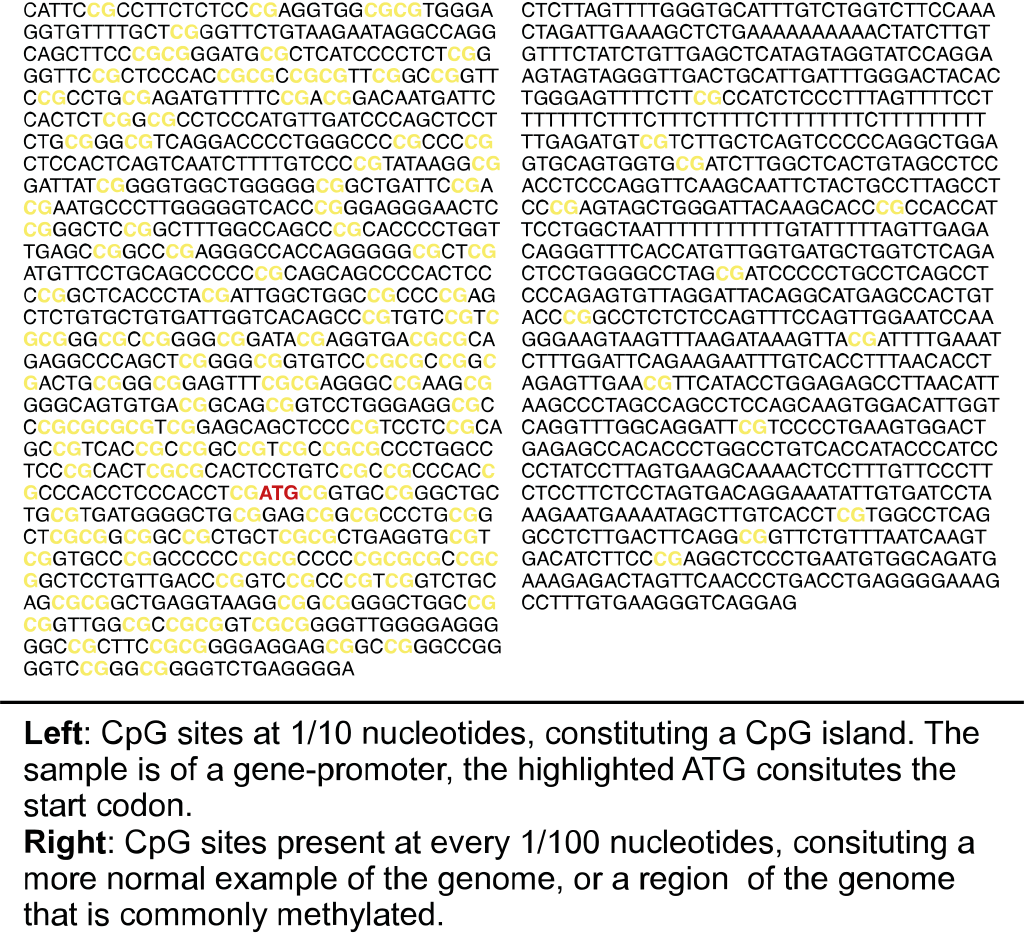
\includegraphics[width=0.8\textwidth]{img/7.png}
        \end{figure}

    \end{frame}
\begin{frame}
    \frametitle{Toy Example \footnote{example from the \href{https://www.cis.upenn.edu/~cis262/notes/Example-Viterbi-DNA.pdf}{link}}}
    
    \begin{figure}[T]
        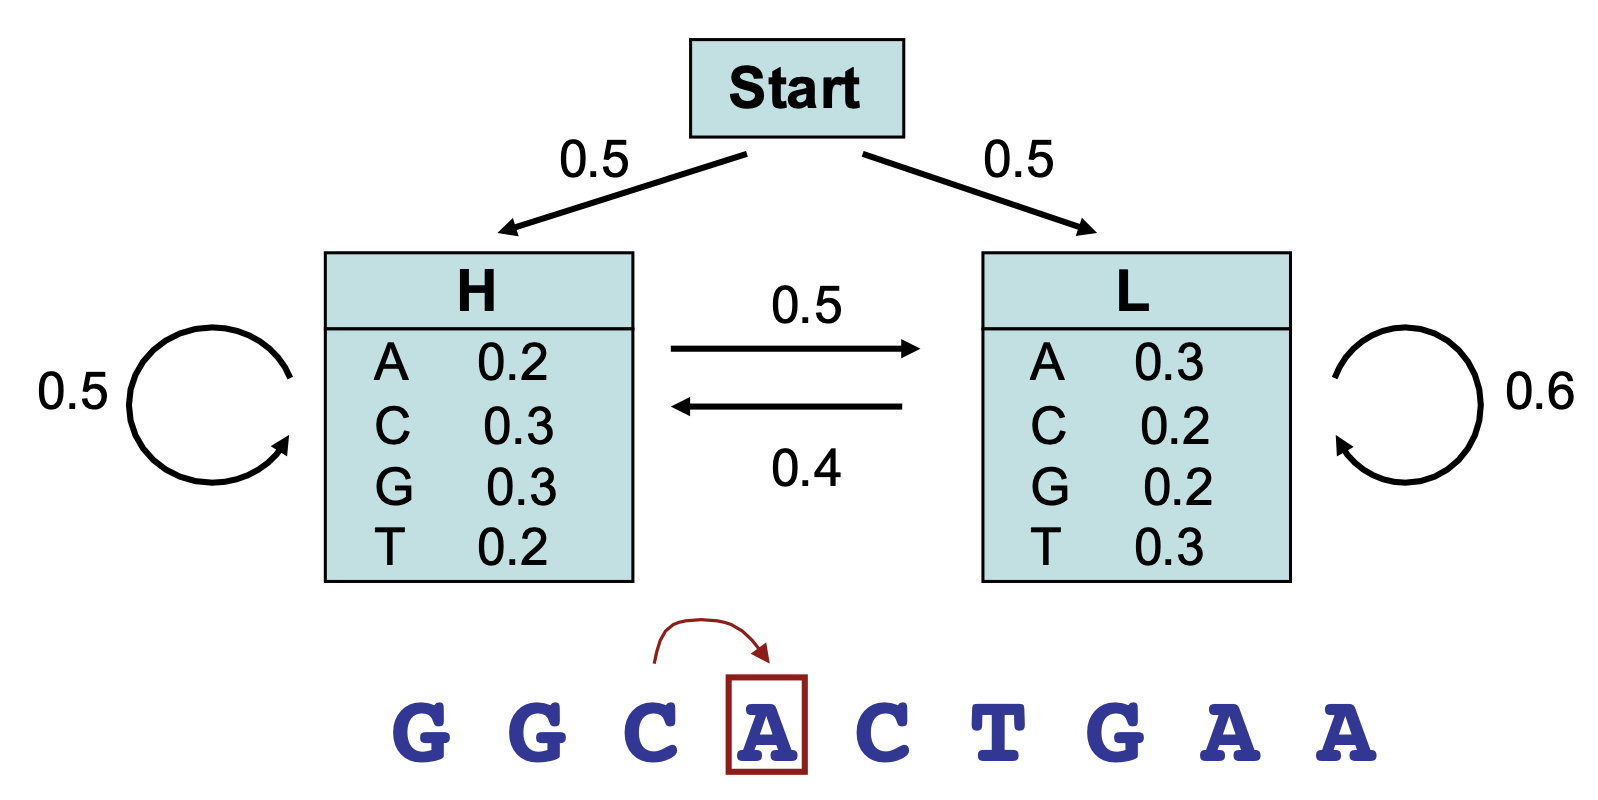
\includegraphics[width=0.8\textwidth]{img/8.png}
        \end{figure}
        This model is composed of 2 states, H (high GC content) and L (low GC content). We can for example consider that state H characterizes coding DNA while L characterizes non-coding DNA.
        $$
        p_{H}(A, 4)=e_{H}(A) \max \left(p_{L}(C, 3) p_{L H}, p_{H}(C, 3) p_{H H}\right)
        $$
    \end{frame}
\begin{frame}
        \frametitle{Toy Example}
        
        \begin{figure}[T]
            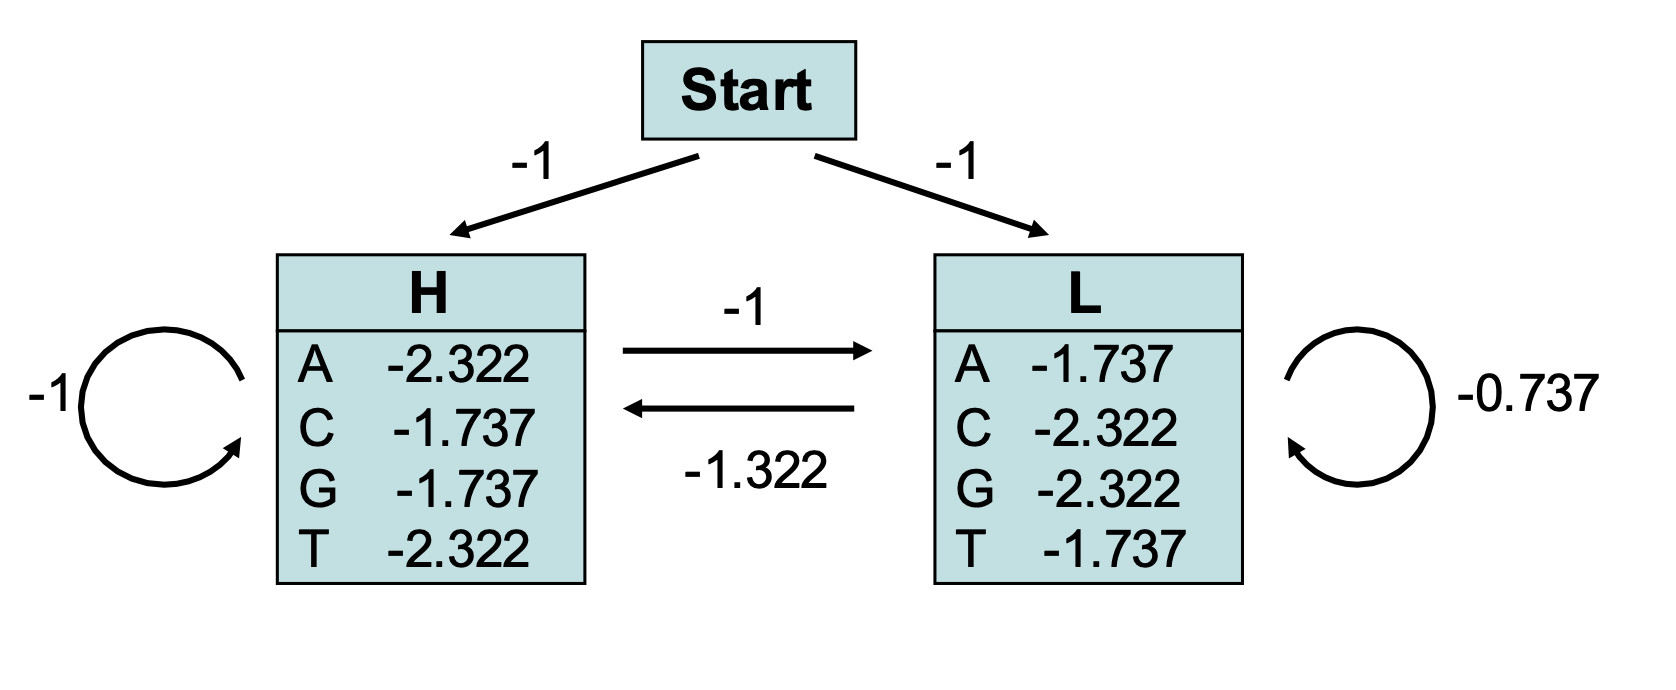
\includegraphics[width=0.8\textwidth]{img/9.png}
            \end{figure}
            We used here $log2(p)$, and compute sums instead of products.
        \end{frame}

\begin{frame}
    \frametitle{Toy Example}
    
    \begin{figure}[T]
        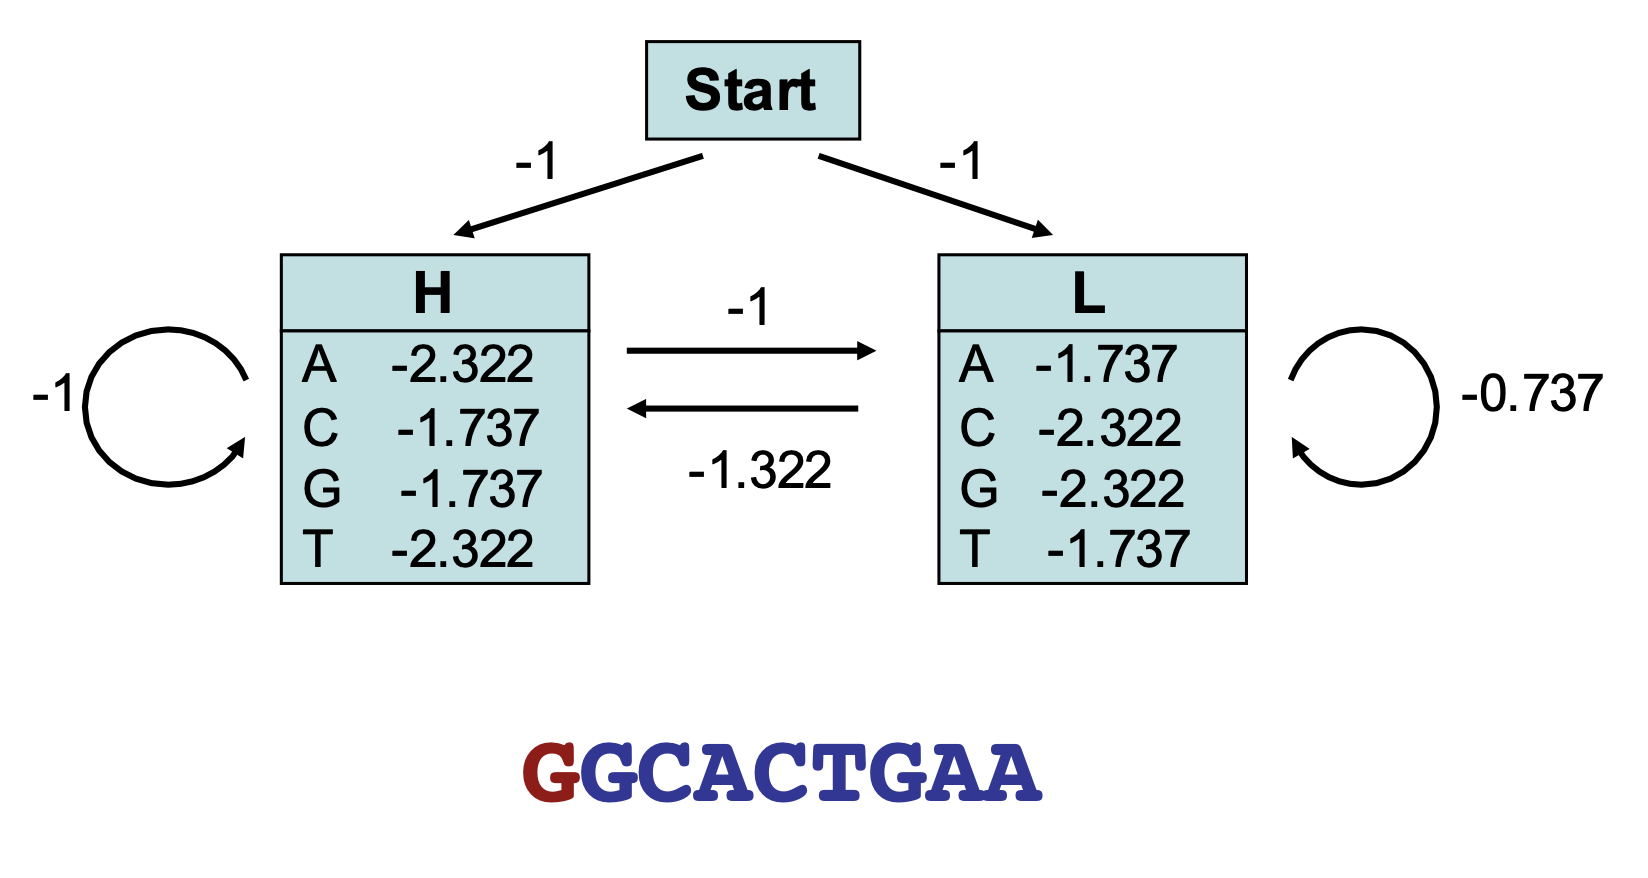
\includegraphics[width=0.8\textwidth]{img/10.png}
        \end{figure}
        \begin{itemize}
            \item         Probability (in $log_2$) that G at the first position was emitted by state H, $p_H(G,1) = -1 -1.737 = -2.737$
            \item         Probability (in $log_2$) that G at the first position was emitted by state L, $p_L(G,1) = -1 -2.322 = -3.322$
        \end{itemize}

    \end{frame}
\begin{frame}
    \frametitle{Toy Example}
    
    \begin{figure}[T]
        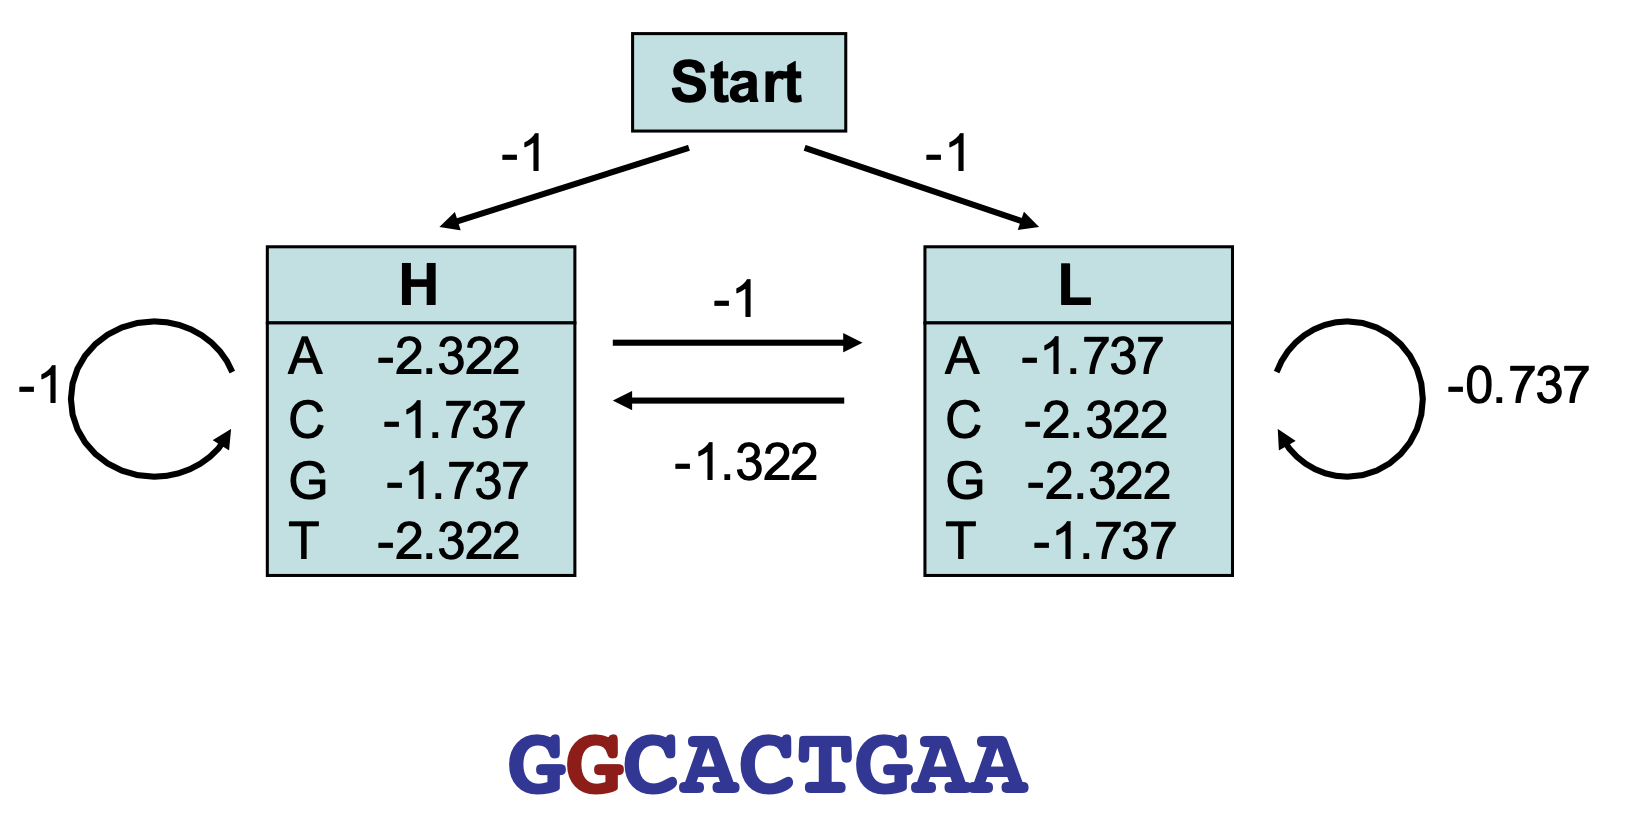
\includegraphics[width=0.8\textwidth]{img/11.png}
        \end{figure}
        \begin{itemize}
            \footnotesize
            \item         Probability (in $log_2$) that G at the 2nd position was emitted by state H, $
        \begin{aligned} p_{H}(G, 2) &=-1.737+\max \left(p_{H}(G, 1)+p_{H H}, p_{L}(G, 1)+p_{L H}\right) \\ &=-1.737+\max (-2.737-1,-3.322-1.322) \\ &=-5.474\left(\text { obtained from } p_{H}(\mathrm{G}, 1)\right) \end{aligned}
        $
            \item         Probability (in $log_2$) that G at the 2nd position was emitted by state L, $
        \begin{aligned} p_{L}(G, 2) &=-2.322+\max \left(p_{H}(G, 1)+p_{H L}, p_{L}(G, 1)+p_{L L}\right) \\ &=-2.322+\max (-2.737-1.322,-3.322-0.737) \\ &=-6.059\left(\text { obtained from } p_{H}(\mathrm{G}, 1)\right) \end{aligned}
        $
        \end{itemize}

    \end{frame}
\begin{frame}
    \frametitle{Toy Example}
    
    \begin{figure}[T]
        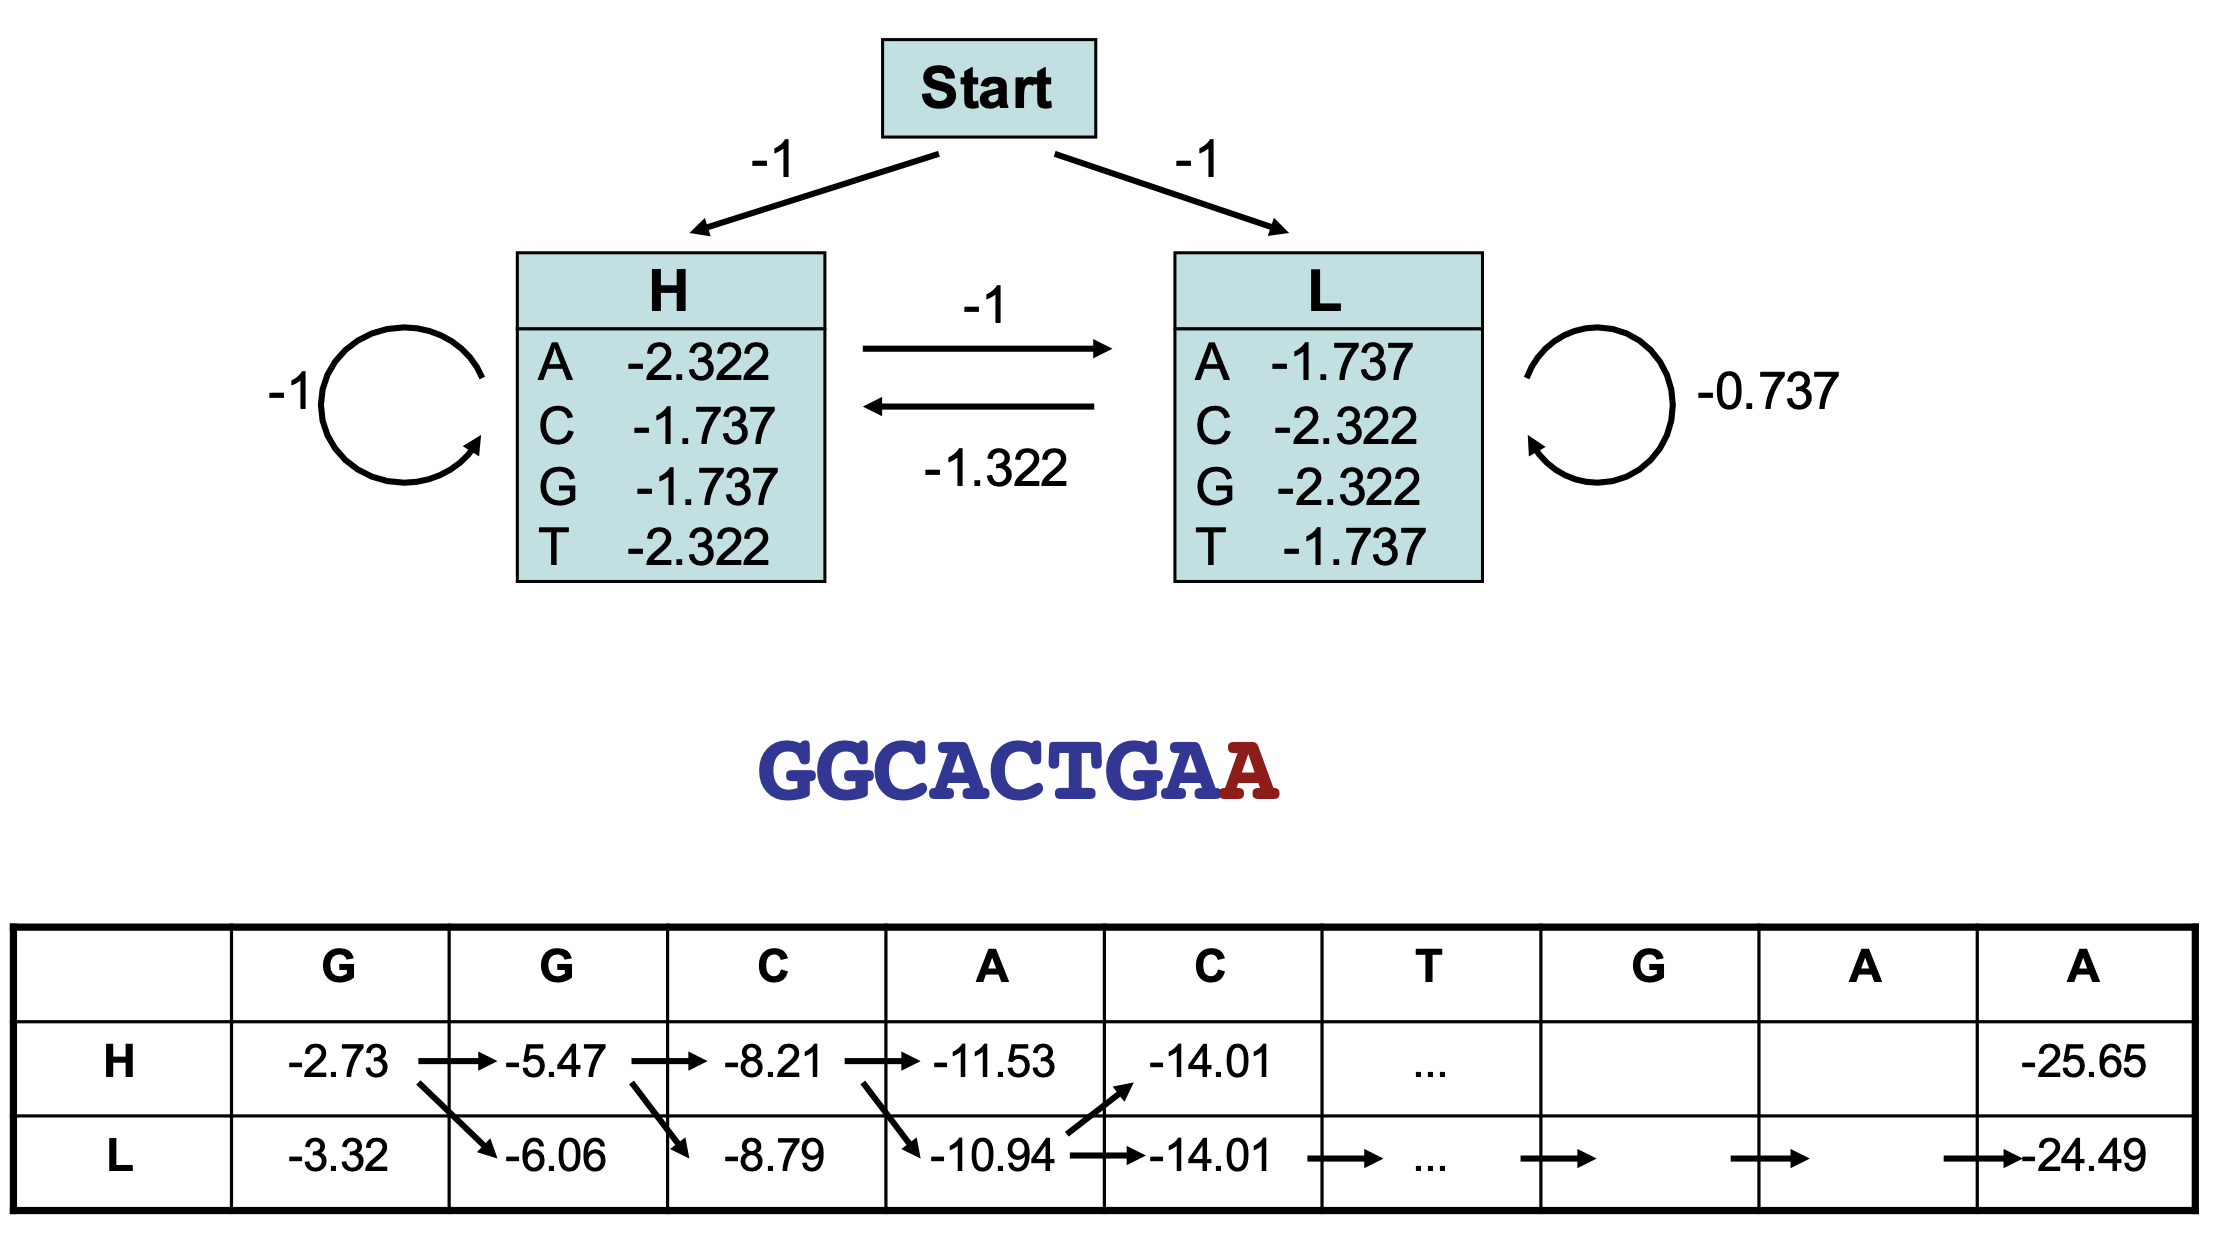
\includegraphics[width=0.8\textwidth]{img/12.png}
        \end{figure}
        We then compute iteratively the probabilities $p_H(i,x)$ and $p_L(i,x)$ that nucleotide i at position x was emitted by state H or L, respectively. 
        The highest probability obtained for the nucleotide at the last position is the probability of the most probable path. 
        This path can be retrieved by back-tracking.

    \end{frame}
\begin{frame}
    \frametitle{Toy Example}
    
    \begin{figure}[T]
        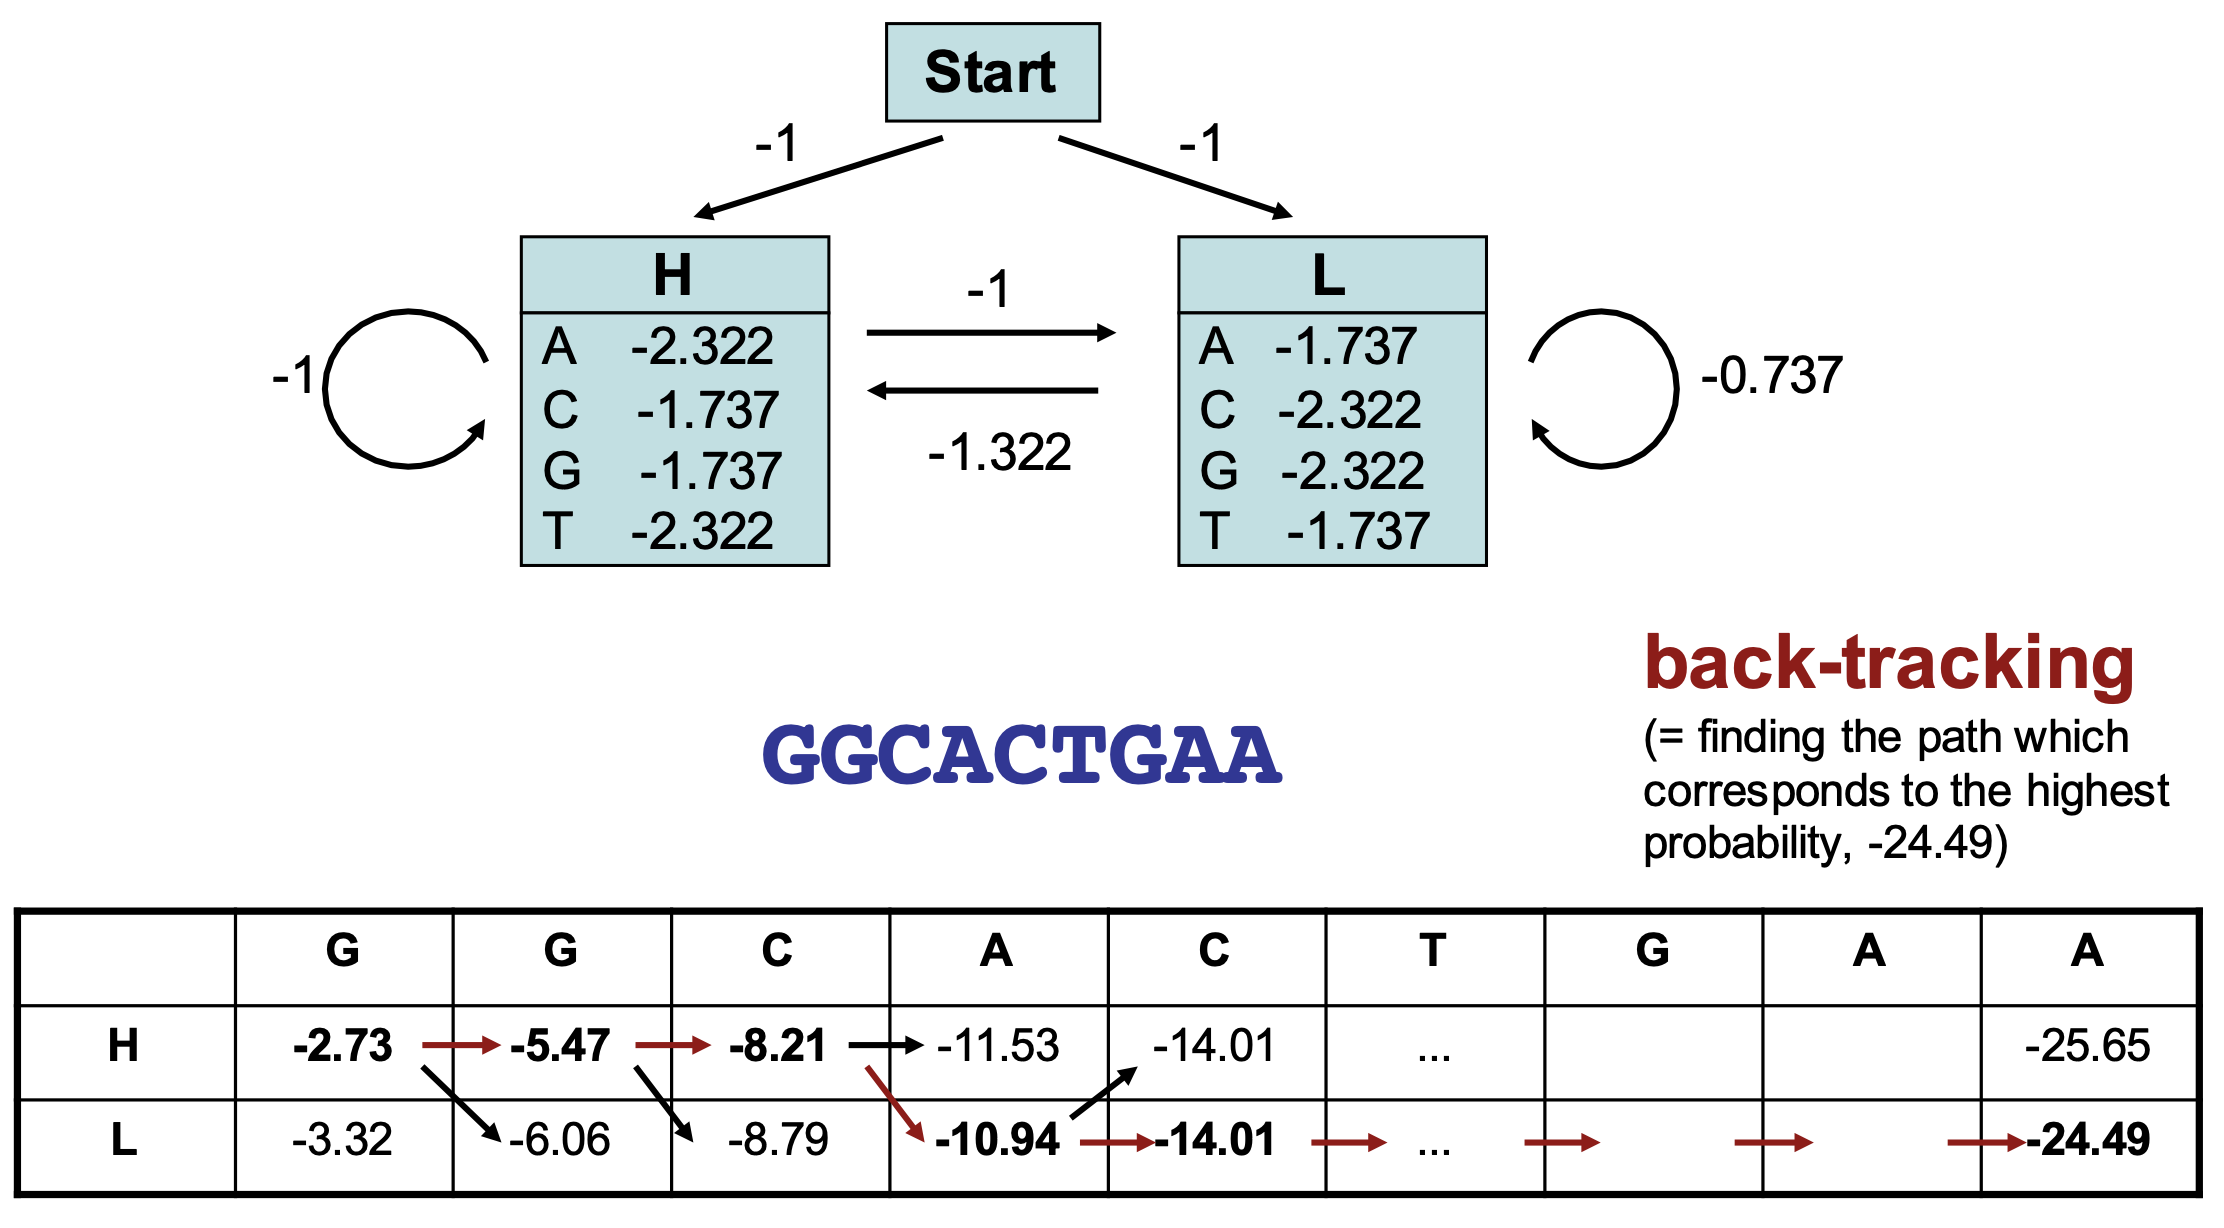
\includegraphics[width=0.8\textwidth]{img/13.png}
        \end{figure}
        The most probable path is: \color{red}HHHLLLLLL

    \end{frame}
\begin{frame}[t, allowframebreaks]
    \frametitle{References}
    \bibliographystyle{amsalpha}
    \bibliography{ref}
    \end{frame}


\end{document}
 
